\section*{04.07.2017}

\paragraph{Allgemein}
\begin{itemize}
	\item Mir ist aufgefallen, dass die \emph{LOOP} in der angedachten Form wenig bringt. Was ich brauche ist nachher $A*x<b$ um darauf die non-term Bedingungen zu prüfen. Aus \emph{main} wird deutlich wie man $A$ und $b$ herleitet. Als: 
		\begin{figure}[H]
			\centering
			$G*x<g \land M*x+m=x'$ \newline
			$A = 
				\begin{pmatrix} 
					G &  0 \\ 
					M & -I \\
					-M & I 
				\end{pmatrix}, b = \begin{pmatrix}
					g \\
					-m \\
					m
				\end{pmatrix}$
		\end{figure}
		Die bisher hergeleitete \emph{Speed}-Matrix kann als $M$ übernommen werden, da es die linearen Updates schreibt. Im folgenden werde ich die Matrizen wie folgt nennen:
		\begin{figure}[H]
			\centering
			\begin{minipage}{0.4\textwidth}
				\begin{description}
					\item $G$: GuardUpdates
					\item $g$: GuardConstants
					\item $M$: UpdateMatrix
				\end{description}
			\end{minipage}
			\begin{minipage}{0.4\textwidth}
				\begin{description}
					\item $m$: UpdateConstants
					\item $A$: IterationMatrix
					\item $b$: IterationConstants
				\end{description}
			\end{minipage}
		\end{figure}
	\item Muss den RPNTree anpassen, damit ich die conditions parsen kann. Vielleicht kann ich die \&\&'s splitten, sodass $n$-conds bleiben. \answer und hat auch genau so funktioniert.
	\item Beobachtung: \begin{description}
		\item Sei $n = \# vars$ dann sind sind $x, x' \in \mathbb{Z}^n$
		\item Demnach muss die Updatematrix $M \in \mathbb{Z}^{n\times n}$, da es die Updates für die Variablen ist und $m \in \mathbb{Z}^n$
		\item Sei $m = \# conditions$
			Somit ist $G \in \mathbb{Z}^{m \times n}$ und $g \in \mathbb{Z}^m$
		\item Somit folgt durch $b = \begin{pmatrix} g \\ -m \\	m \end{pmatrix} = \begin{pmatrix} \mathbb{Z}^m \\ \mathbb{Z}^n \\ \mathbb{Z}^n \end{pmatrix} \in \mathbb{Z}^{2*n+m}$,
			dass \newline $A = 
			\begin{pmatrix} 
				G &  0 \\ 
				M & -I \\
				-M & I 
			\end{pmatrix} = \begin{pmatrix} 
			\mathbb{Z}^{m\times n} &  \{0\}^{n\times n} \\ 
			\mathbb{Z}^{n\times n} & I^{n\times n} \\
			\mathbb{Z}^{n\times n} & I^{n\times n} 
			\end{pmatrix} \in \mathbb{Z}^{2*n+m\times 2*n}$.
		\end{description}
	\item Habe die GuardMatrix und die GuardConstants auslesen lassen. Jedoch siehe Problem 3.
	\item Änderungen der Methoden und Attribute in dem \emph{ReversePolishNotationTree}-Package
		\begin{figure}[H]
			% Graphic for TeX using PGF
% Title: D:\Dokumente\GitHub\Bachelorarbeit\Arbeitstagebuch\src\04.07.2017-RPNTree-classdiagram.dia
% Creator: Dia v0.97.2
% CreationDate: Wed Jul 05 10:55:37 2017
% For: Timo Bergerbusch
% \usepackage{tikz}
% The following commands are not supported in PSTricks at present
% We define them conditionally, so when they are implemented,
% this pgf file will use them.
\ifx\du\undefined
  \newlength{\du}
\fi
\setlength{\du}{15\unitlength}
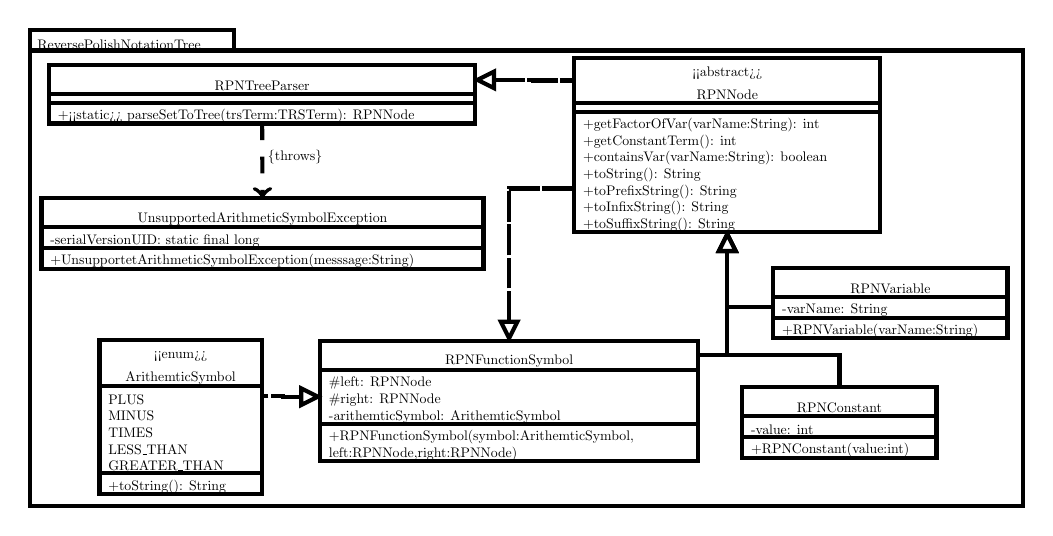
\begin{tikzpicture}[scale=0.5, every node/.style={scale=0.5}]
\pgftransformxscale{1.000000}
\pgftransformyscale{-1.000000}
\definecolor{dialinecolor}{rgb}{0.000000, 0.000000, 0.000000}
\pgfsetstrokecolor{dialinecolor}
\definecolor{dialinecolor}{rgb}{1.000000, 1.000000, 1.000000}
\pgfsetfillcolor{dialinecolor}
\pgfsetlinewidth{0.100000\du}
\pgfsetdash{}{0pt}
\definecolor{dialinecolor}{rgb}{1.000000, 1.000000, 1.000000}
\pgfsetfillcolor{dialinecolor}
\fill (-2.412994\du,34.090870\du)--(-2.412994\du,56.028781\du)--(45.422570\du,56.028781\du)--(45.422570\du,34.090870\du)--cycle;
\definecolor{dialinecolor}{rgb}{0.000000, 0.000000, 0.000000}
\pgfsetstrokecolor{dialinecolor}
\draw (-2.412994\du,34.090870\du)--(-2.412994\du,56.028781\du)--(45.422570\du,56.028781\du)--(45.422570\du,34.090870\du)--cycle;
\definecolor{dialinecolor}{rgb}{1.000000, 1.000000, 1.000000}
\pgfsetfillcolor{dialinecolor}
\fill (-2.412994\du,33.090870\du)--(-2.412994\du,34.090870\du)--(7.412006\du,34.090870\du)--(7.412006\du,33.090870\du)--cycle;
\definecolor{dialinecolor}{rgb}{0.000000, 0.000000, 0.000000}
\pgfsetstrokecolor{dialinecolor}
\draw (-2.412994\du,33.090870\du)--(-2.412994\du,34.090870\du)--(7.412006\du,34.090870\du)--(7.412006\du,33.090870\du)--cycle;
% setfont left to latex
\definecolor{dialinecolor}{rgb}{0.000000, 0.000000, 0.000000}
\pgfsetstrokecolor{dialinecolor}
\node[anchor=west] at (-2.312994\du,33.790870\du){ReversePolishNotationTree};
\pgfsetlinewidth{0.100000\du}
\pgfsetdash{}{0pt}
\definecolor{dialinecolor}{rgb}{1.000000, 1.000000, 1.000000}
\pgfsetfillcolor{dialinecolor}
\fill (23.823426\du,34.435422\du)--(23.823426\du,36.635422\du)--(38.568426\du,36.635422\du)--(38.568426\du,34.435422\du)--cycle;
\definecolor{dialinecolor}{rgb}{0.000000, 0.000000, 0.000000}
\pgfsetstrokecolor{dialinecolor}
\draw (23.823426\du,34.435422\du)--(23.823426\du,36.635422\du)--(38.568426\du,36.635422\du)--(38.568426\du,34.435422\du)--cycle;
% setfont left to latex
\definecolor{dialinecolor}{rgb}{0.000000, 0.000000, 0.000000}
\pgfsetstrokecolor{dialinecolor}
\node at (31.195926\du,35.195422\du){<<abstract>>};
% setfont left to latex
\definecolor{dialinecolor}{rgb}{0.000000, 0.000000, 0.000000}
\pgfsetstrokecolor{dialinecolor}
\node at (31.195926\du,36.235422\du){RPNNode};
\definecolor{dialinecolor}{rgb}{1.000000, 1.000000, 1.000000}
\pgfsetfillcolor{dialinecolor}
\fill (23.823426\du,36.635422\du)--(23.823426\du,37.035422\du)--(38.568426\du,37.035422\du)--(38.568426\du,36.635422\du)--cycle;
\definecolor{dialinecolor}{rgb}{0.000000, 0.000000, 0.000000}
\pgfsetstrokecolor{dialinecolor}
\draw (23.823426\du,36.635422\du)--(23.823426\du,37.035422\du)--(38.568426\du,37.035422\du)--(38.568426\du,36.635422\du)--cycle;
\definecolor{dialinecolor}{rgb}{1.000000, 1.000000, 1.000000}
\pgfsetfillcolor{dialinecolor}
\fill (23.823426\du,37.035422\du)--(23.823426\du,42.835422\du)--(38.568426\du,42.835422\du)--(38.568426\du,37.035422\du)--cycle;
\definecolor{dialinecolor}{rgb}{0.000000, 0.000000, 0.000000}
\pgfsetstrokecolor{dialinecolor}
\draw (23.823426\du,37.035422\du)--(23.823426\du,42.835422\du)--(38.568426\du,42.835422\du)--(38.568426\du,37.035422\du)--cycle;
% setfont left to latex
\definecolor{dialinecolor}{rgb}{0.000000, 0.000000, 0.000000}
\pgfsetstrokecolor{dialinecolor}
\node[anchor=west] at (23.973426\du,37.695422\du){+getFactorOfVar(varName:String): int};
% setfont left to latex
\definecolor{dialinecolor}{rgb}{0.000000, 0.000000, 0.000000}
\pgfsetstrokecolor{dialinecolor}
\node[anchor=west] at (23.973426\du,38.495422\du){+getConstantTerm(): int};
% setfont left to latex
\definecolor{dialinecolor}{rgb}{0.000000, 0.000000, 0.000000}
\pgfsetstrokecolor{dialinecolor}
\node[anchor=west] at (23.973426\du,39.295422\du){+containsVar(varName:String): boolean};
% setfont left to latex
\definecolor{dialinecolor}{rgb}{0.000000, 0.000000, 0.000000}
\pgfsetstrokecolor{dialinecolor}
\node[anchor=west] at (23.973426\du,40.095422\du){+toString(): String};
% setfont left to latex
\definecolor{dialinecolor}{rgb}{0.000000, 0.000000, 0.000000}
\pgfsetstrokecolor{dialinecolor}
\node[anchor=west] at (23.973426\du,40.895422\du){+toPrefixString(): String};
% setfont left to latex
\definecolor{dialinecolor}{rgb}{0.000000, 0.000000, 0.000000}
\pgfsetstrokecolor{dialinecolor}
\node[anchor=west] at (23.973426\du,41.695422\du){+toInfixString(): String};
% setfont left to latex
\definecolor{dialinecolor}{rgb}{0.000000, 0.000000, 0.000000}
\pgfsetstrokecolor{dialinecolor}
\node[anchor=west] at (23.973426\du,42.495422\du){+toSuffixString(): String};
\pgfsetlinewidth{0.100000\du}
\pgfsetdash{}{0pt}
\definecolor{dialinecolor}{rgb}{1.000000, 1.000000, 1.000000}
\pgfsetfillcolor{dialinecolor}
\fill (33.415475\du,44.559641\du)--(33.415475\du,45.959641\du)--(44.695475\du,45.959641\du)--(44.695475\du,44.559641\du)--cycle;
\definecolor{dialinecolor}{rgb}{0.000000, 0.000000, 0.000000}
\pgfsetstrokecolor{dialinecolor}
\draw (33.415475\du,44.559641\du)--(33.415475\du,45.959641\du)--(44.695475\du,45.959641\du)--(44.695475\du,44.559641\du)--cycle;
% setfont left to latex
\definecolor{dialinecolor}{rgb}{0.000000, 0.000000, 0.000000}
\pgfsetstrokecolor{dialinecolor}
\node at (39.055475\du,45.559641\du){RPNVariable};
\definecolor{dialinecolor}{rgb}{1.000000, 1.000000, 1.000000}
\pgfsetfillcolor{dialinecolor}
\fill (33.415475\du,45.959641\du)--(33.415475\du,46.959641\du)--(44.695475\du,46.959641\du)--(44.695475\du,45.959641\du)--cycle;
\definecolor{dialinecolor}{rgb}{0.000000, 0.000000, 0.000000}
\pgfsetstrokecolor{dialinecolor}
\draw (33.415475\du,45.959641\du)--(33.415475\du,46.959641\du)--(44.695475\du,46.959641\du)--(44.695475\du,45.959641\du)--cycle;
% setfont left to latex
\definecolor{dialinecolor}{rgb}{0.000000, 0.000000, 0.000000}
\pgfsetstrokecolor{dialinecolor}
\node[anchor=west] at (33.565475\du,46.619641\du){-varName: String};
\definecolor{dialinecolor}{rgb}{1.000000, 1.000000, 1.000000}
\pgfsetfillcolor{dialinecolor}
\fill (33.415475\du,46.959641\du)--(33.415475\du,47.959641\du)--(44.695475\du,47.959641\du)--(44.695475\du,46.959641\du)--cycle;
\definecolor{dialinecolor}{rgb}{0.000000, 0.000000, 0.000000}
\pgfsetstrokecolor{dialinecolor}
\draw (33.415475\du,46.959641\du)--(33.415475\du,47.959641\du)--(44.695475\du,47.959641\du)--(44.695475\du,46.959641\du)--cycle;
% setfont left to latex
\definecolor{dialinecolor}{rgb}{0.000000, 0.000000, 0.000000}
\pgfsetstrokecolor{dialinecolor}
\node[anchor=west] at (33.565475\du,47.619641\du){+RPNVariable(varName:String)};
\pgfsetlinewidth{0.100000\du}
\pgfsetdash{}{0pt}
\definecolor{dialinecolor}{rgb}{1.000000, 1.000000, 1.000000}
\pgfsetfillcolor{dialinecolor}
\fill (31.921154\du,50.304367\du)--(31.921154\du,51.704367\du)--(41.276154\du,51.704367\du)--(41.276154\du,50.304367\du)--cycle;
\definecolor{dialinecolor}{rgb}{0.000000, 0.000000, 0.000000}
\pgfsetstrokecolor{dialinecolor}
\draw (31.921154\du,50.304367\du)--(31.921154\du,51.704367\du)--(41.276154\du,51.704367\du)--(41.276154\du,50.304367\du)--cycle;
% setfont left to latex
\definecolor{dialinecolor}{rgb}{0.000000, 0.000000, 0.000000}
\pgfsetstrokecolor{dialinecolor}
\node at (36.598654\du,51.304367\du){RPNConstant};
\definecolor{dialinecolor}{rgb}{1.000000, 1.000000, 1.000000}
\pgfsetfillcolor{dialinecolor}
\fill (31.921154\du,51.704367\du)--(31.921154\du,52.704367\du)--(41.276154\du,52.704367\du)--(41.276154\du,51.704367\du)--cycle;
\definecolor{dialinecolor}{rgb}{0.000000, 0.000000, 0.000000}
\pgfsetstrokecolor{dialinecolor}
\draw (31.921154\du,51.704367\du)--(31.921154\du,52.704367\du)--(41.276154\du,52.704367\du)--(41.276154\du,51.704367\du)--cycle;
% setfont left to latex
\definecolor{dialinecolor}{rgb}{0.000000, 0.000000, 0.000000}
\pgfsetstrokecolor{dialinecolor}
\node[anchor=west] at (32.071154\du,52.364367\du){-value: int};
\definecolor{dialinecolor}{rgb}{1.000000, 1.000000, 1.000000}
\pgfsetfillcolor{dialinecolor}
\fill (31.921154\du,52.704367\du)--(31.921154\du,53.704367\du)--(41.276154\du,53.704367\du)--(41.276154\du,52.704367\du)--cycle;
\definecolor{dialinecolor}{rgb}{0.000000, 0.000000, 0.000000}
\pgfsetstrokecolor{dialinecolor}
\draw (31.921154\du,52.704367\du)--(31.921154\du,53.704367\du)--(41.276154\du,53.704367\du)--(41.276154\du,52.704367\du)--cycle;
% setfont left to latex
\definecolor{dialinecolor}{rgb}{0.000000, 0.000000, 0.000000}
\pgfsetstrokecolor{dialinecolor}
\node[anchor=west] at (32.071154\du,53.364367\du){+RPNConstant(value:int)};
\pgfsetlinewidth{0.100000\du}
\pgfsetdash{}{0pt}
\definecolor{dialinecolor}{rgb}{1.000000, 1.000000, 1.000000}
\pgfsetfillcolor{dialinecolor}
\fill (11.578208\du,48.068165\du)--(11.578208\du,49.468165\du)--(29.788208\du,49.468165\du)--(29.788208\du,48.068165\du)--cycle;
\definecolor{dialinecolor}{rgb}{0.000000, 0.000000, 0.000000}
\pgfsetstrokecolor{dialinecolor}
\draw (11.578208\du,48.068165\du)--(11.578208\du,49.468165\du)--(29.788208\du,49.468165\du)--(29.788208\du,48.068165\du)--cycle;
% setfont left to latex
\definecolor{dialinecolor}{rgb}{0.000000, 0.000000, 0.000000}
\pgfsetstrokecolor{dialinecolor}
\node at (20.683208\du,49.068165\du){RPNFunctionSymbol};
\definecolor{dialinecolor}{rgb}{1.000000, 1.000000, 1.000000}
\pgfsetfillcolor{dialinecolor}
\fill (11.578208\du,49.468165\du)--(11.578208\du,52.068165\du)--(29.788208\du,52.068165\du)--(29.788208\du,49.468165\du)--cycle;
\definecolor{dialinecolor}{rgb}{0.000000, 0.000000, 0.000000}
\pgfsetstrokecolor{dialinecolor}
\draw (11.578208\du,49.468165\du)--(11.578208\du,52.068165\du)--(29.788208\du,52.068165\du)--(29.788208\du,49.468165\du)--cycle;
% setfont left to latex
\definecolor{dialinecolor}{rgb}{0.000000, 0.000000, 0.000000}
\pgfsetstrokecolor{dialinecolor}
\node[anchor=west] at (11.728208\du,50.128165\du){\#left: RPNNode};
% setfont left to latex
\definecolor{dialinecolor}{rgb}{0.000000, 0.000000, 0.000000}
\pgfsetstrokecolor{dialinecolor}
\node[anchor=west] at (11.728208\du,50.928165\du){\#right: RPNNode};
% setfont left to latex
\definecolor{dialinecolor}{rgb}{0.000000, 0.000000, 0.000000}
\pgfsetstrokecolor{dialinecolor}
\node[anchor=west] at (11.728208\du,51.728165\du){-arithemticSymbol: ArithemticSymbol};
\definecolor{dialinecolor}{rgb}{1.000000, 1.000000, 1.000000}
\pgfsetfillcolor{dialinecolor}
\fill (11.578208\du,52.068165\du)--(11.578208\du,53.868165\du)--(29.788208\du,53.868165\du)--(29.788208\du,52.068165\du)--cycle;
\definecolor{dialinecolor}{rgb}{0.000000, 0.000000, 0.000000}
\pgfsetstrokecolor{dialinecolor}
\draw (11.578208\du,52.068165\du)--(11.578208\du,53.868165\du)--(29.788208\du,53.868165\du)--(29.788208\du,52.068165\du)--cycle;
% setfont left to latex
\definecolor{dialinecolor}{rgb}{0.000000, 0.000000, 0.000000}
\pgfsetstrokecolor{dialinecolor}
\node[anchor=west] at (11.728208\du,52.728165\du){+RPNFunctionSymbol(symbol:ArithemticSymbol,};
\definecolor{dialinecolor}{rgb}{0.000000, 0.000000, 0.000000}
\pgfsetstrokecolor{dialinecolor}
\node[anchor=west] at (11.728208\du,53.528165\du){                   left:RPNNode,right:RPNNode)};
\pgfsetlinewidth{0.100000\du}
\pgfsetdash{}{0pt}
\pgfsetmiterjoin
\pgfsetbuttcap
{
\definecolor{dialinecolor}{rgb}{0.000000, 0.000000, 0.000000}
\pgfsetfillcolor{dialinecolor}
% was here!!!
\definecolor{dialinecolor}{rgb}{0.000000, 0.000000, 0.000000}
\pgfsetstrokecolor{dialinecolor}
\draw (31.195926\du,42.835422\du)--(31.195926\du,46.459641\du)--(33.415475\du,46.459641\du);
}
\definecolor{dialinecolor}{rgb}{0.000000, 0.000000, 0.000000}
\pgfsetstrokecolor{dialinecolor}
\draw (31.195926\du,43.747226\du)--(31.195926\du,46.459641\du)--(33.415475\du,46.459641\du);
\pgfsetmiterjoin
\definecolor{dialinecolor}{rgb}{1.000000, 1.000000, 1.000000}
\pgfsetfillcolor{dialinecolor}
\fill (31.595926\du,43.747226\du)--(31.195926\du,42.947226\du)--(30.795926\du,43.747226\du)--cycle;
\pgfsetlinewidth{0.100000\du}
\pgfsetdash{}{0pt}
\pgfsetmiterjoin
\definecolor{dialinecolor}{rgb}{0.000000, 0.000000, 0.000000}
\pgfsetstrokecolor{dialinecolor}
\draw (31.595926\du,43.747226\du)--(31.195926\du,42.947226\du)--(30.795926\du,43.747226\du)--cycle;
% setfont left to latex
\pgfsetlinewidth{0.100000\du}
\pgfsetdash{}{0pt}
\pgfsetmiterjoin
\pgfsetbuttcap
{
\definecolor{dialinecolor}{rgb}{0.000000, 0.000000, 0.000000}
\pgfsetfillcolor{dialinecolor}
% was here!!!
\definecolor{dialinecolor}{rgb}{0.000000, 0.000000, 0.000000}
\pgfsetstrokecolor{dialinecolor}
\draw (31.195926\du,42.835422\du)--(31.195926\du,48.780402\du)--(36.598654\du,48.780402\du)--(36.598654\du,50.304367\du);
}
\definecolor{dialinecolor}{rgb}{0.000000, 0.000000, 0.000000}
\pgfsetstrokecolor{dialinecolor}
\draw (31.195926\du,43.747226\du)--(31.195926\du,48.780402\du)--(36.598654\du,48.780402\du)--(36.598654\du,50.304367\du);
\pgfsetmiterjoin
\definecolor{dialinecolor}{rgb}{1.000000, 1.000000, 1.000000}
\pgfsetfillcolor{dialinecolor}
\fill (31.595926\du,43.747226\du)--(31.195926\du,42.947226\du)--(30.795926\du,43.747226\du)--cycle;
\pgfsetlinewidth{0.100000\du}
\pgfsetdash{}{0pt}
\pgfsetmiterjoin
\definecolor{dialinecolor}{rgb}{0.000000, 0.000000, 0.000000}
\pgfsetstrokecolor{dialinecolor}
\draw (31.595926\du,43.747226\du)--(31.195926\du,42.947226\du)--(30.795926\du,43.747226\du)--cycle;
% setfont left to latex
\pgfsetlinewidth{0.100000\du}
\pgfsetdash{}{0pt}
\pgfsetmiterjoin
\pgfsetbuttcap
{
\definecolor{dialinecolor}{rgb}{0.000000, 0.000000, 0.000000}
\pgfsetfillcolor{dialinecolor}
% was here!!!
\definecolor{dialinecolor}{rgb}{0.000000, 0.000000, 0.000000}
\pgfsetstrokecolor{dialinecolor}
\draw (31.195926\du,42.835422\du)--(31.195926\du,48.768165\du)--(29.788208\du,48.768165\du);
}
\definecolor{dialinecolor}{rgb}{0.000000, 0.000000, 0.000000}
\pgfsetstrokecolor{dialinecolor}
\draw (31.195926\du,43.747226\du)--(31.195926\du,48.768165\du)--(29.788208\du,48.768165\du);
\pgfsetmiterjoin
\definecolor{dialinecolor}{rgb}{1.000000, 1.000000, 1.000000}
\pgfsetfillcolor{dialinecolor}
\fill (31.595926\du,43.747226\du)--(31.195926\du,42.947226\du)--(30.795926\du,43.747226\du)--cycle;
\pgfsetlinewidth{0.100000\du}
\pgfsetdash{}{0pt}
\pgfsetmiterjoin
\definecolor{dialinecolor}{rgb}{0.000000, 0.000000, 0.000000}
\pgfsetstrokecolor{dialinecolor}
\draw (31.595926\du,43.747226\du)--(31.195926\du,42.947226\du)--(30.795926\du,43.747226\du)--cycle;
% setfont left to latex
\pgfsetlinewidth{0.100000\du}
\pgfsetdash{}{0pt}
\definecolor{dialinecolor}{rgb}{1.000000, 1.000000, 1.000000}
\pgfsetfillcolor{dialinecolor}
\fill (0.948979\du,48.048596\du)--(0.948979\du,50.248596\du)--(8.763979\du,50.248596\du)--(8.763979\du,48.048596\du)--cycle;
\definecolor{dialinecolor}{rgb}{0.000000, 0.000000, 0.000000}
\pgfsetstrokecolor{dialinecolor}
\draw (0.948979\du,48.048596\du)--(0.948979\du,50.248596\du)--(8.763979\du,50.248596\du)--(8.763979\du,48.048596\du)--cycle;
% setfont left to latex
\definecolor{dialinecolor}{rgb}{0.000000, 0.000000, 0.000000}
\pgfsetstrokecolor{dialinecolor}
\node at (4.856479\du,48.808596\du){<<enum>>};
% setfont left to latex
\definecolor{dialinecolor}{rgb}{0.000000, 0.000000, 0.000000}
\pgfsetstrokecolor{dialinecolor}
\node at (4.856479\du,49.848596\du){ArithemticSymbol};
\definecolor{dialinecolor}{rgb}{1.000000, 1.000000, 1.000000}
\pgfsetfillcolor{dialinecolor}
\fill (0.948979\du,50.248596\du)--(0.948979\du,54.448596\du)--(8.763979\du,54.448596\du)--(8.763979\du,50.248596\du)--cycle;
\definecolor{dialinecolor}{rgb}{0.000000, 0.000000, 0.000000}
\pgfsetstrokecolor{dialinecolor}
\draw (0.948979\du,50.248596\du)--(0.948979\du,54.448596\du)--(8.763979\du,54.448596\du)--(8.763979\du,50.248596\du)--cycle;
% setfont left to latex
\definecolor{dialinecolor}{rgb}{0.000000, 0.000000, 0.000000}
\pgfsetstrokecolor{dialinecolor}
\node[anchor=west] at (1.098979\du,50.908596\du){ PLUS};
% setfont left to latex
\definecolor{dialinecolor}{rgb}{0.000000, 0.000000, 0.000000}
\pgfsetstrokecolor{dialinecolor}
\node[anchor=west] at (1.098979\du,51.708596\du){ MINUS};
% setfont left to latex
\definecolor{dialinecolor}{rgb}{0.000000, 0.000000, 0.000000}
\pgfsetstrokecolor{dialinecolor}
\node[anchor=west] at (1.098979\du,52.508596\du){ TIMES};
% setfont left to latex
\definecolor{dialinecolor}{rgb}{0.000000, 0.000000, 0.000000}
\pgfsetstrokecolor{dialinecolor}
\node[anchor=west] at (1.098979\du,53.308596\du){ LESS\_THAN};
% setfont left to latex
\definecolor{dialinecolor}{rgb}{0.000000, 0.000000, 0.000000}
\pgfsetstrokecolor{dialinecolor}
\node[anchor=west] at (1.098979\du,54.108596\du){ GREATER\_THAN};
\definecolor{dialinecolor}{rgb}{1.000000, 1.000000, 1.000000}
\pgfsetfillcolor{dialinecolor}
\fill (0.948979\du,54.448596\du)--(0.948979\du,55.448596\du)--(8.763979\du,55.448596\du)--(8.763979\du,54.448596\du)--cycle;
\definecolor{dialinecolor}{rgb}{0.000000, 0.000000, 0.000000}
\pgfsetstrokecolor{dialinecolor}
\draw (0.948979\du,54.448596\du)--(0.948979\du,55.448596\du)--(8.763979\du,55.448596\du)--(8.763979\du,54.448596\du)--cycle;
% setfont left to latex
\definecolor{dialinecolor}{rgb}{0.000000, 0.000000, 0.000000}
\pgfsetstrokecolor{dialinecolor}
\node[anchor=west] at (1.098979\du,55.108596\du){+toString(): String};
\pgfsetlinewidth{0.100000\du}
\pgfsetdash{{1.000000\du}{1.000000\du}}{0\du}
\pgfsetdash{{0.400000\du}{0.400000\du}}{0\du}
\pgfsetmiterjoin
\pgfsetbuttcap
{
\definecolor{dialinecolor}{rgb}{0.000000, 0.000000, 0.000000}
\pgfsetfillcolor{dialinecolor}
% was here!!!
\definecolor{dialinecolor}{rgb}{0.000000, 0.000000, 0.000000}
\pgfsetstrokecolor{dialinecolor}
\draw (11.578208\du,50.768165\du)--(9.771094\du,50.768165\du)--(9.771094\du,50.748596\du)--(8.763979\du,50.748596\du);
}
\definecolor{dialinecolor}{rgb}{0.000000, 0.000000, 0.000000}
\pgfsetstrokecolor{dialinecolor}
\draw (10.666405\du,50.768165\du)--(9.771094\du,50.768165\du)--(9.771094\du,50.748596\du)--(8.763979\du,50.748596\du);
\pgfsetmiterjoin
\definecolor{dialinecolor}{rgb}{1.000000, 1.000000, 1.000000}
\pgfsetfillcolor{dialinecolor}
\fill (10.666405\du,51.168165\du)--(11.466405\du,50.768165\du)--(10.666405\du,50.368165\du)--cycle;
\pgfsetlinewidth{0.100000\du}
\pgfsetdash{}{0pt}
\pgfsetmiterjoin
\definecolor{dialinecolor}{rgb}{0.000000, 0.000000, 0.000000}
\pgfsetstrokecolor{dialinecolor}
\draw (10.666405\du,51.168165\du)--(11.466405\du,50.768165\du)--(10.666405\du,50.368165\du)--cycle;
% setfont left to latex
\pgfsetlinewidth{0.100000\du}
\pgfsetdash{}{0pt}
\definecolor{dialinecolor}{rgb}{1.000000, 1.000000, 1.000000}
\pgfsetfillcolor{dialinecolor}
\fill (-1.476290\du,34.805480\du)--(-1.476290\du,36.205480\du)--(19.043710\du,36.205480\du)--(19.043710\du,34.805480\du)--cycle;
\definecolor{dialinecolor}{rgb}{0.000000, 0.000000, 0.000000}
\pgfsetstrokecolor{dialinecolor}
\draw (-1.476290\du,34.805480\du)--(-1.476290\du,36.205480\du)--(19.043710\du,36.205480\du)--(19.043710\du,34.805480\du)--cycle;
% setfont left to latex
\definecolor{dialinecolor}{rgb}{0.000000, 0.000000, 0.000000}
\pgfsetstrokecolor{dialinecolor}
\node at (8.783710\du,35.805480\du){RPNTreeParser};
\definecolor{dialinecolor}{rgb}{1.000000, 1.000000, 1.000000}
\pgfsetfillcolor{dialinecolor}
\fill (-1.476290\du,36.205480\du)--(-1.476290\du,36.605480\du)--(19.043710\du,36.605480\du)--(19.043710\du,36.205480\du)--cycle;
\definecolor{dialinecolor}{rgb}{0.000000, 0.000000, 0.000000}
\pgfsetstrokecolor{dialinecolor}
\draw (-1.476290\du,36.205480\du)--(-1.476290\du,36.605480\du)--(19.043710\du,36.605480\du)--(19.043710\du,36.205480\du)--cycle;
\definecolor{dialinecolor}{rgb}{1.000000, 1.000000, 1.000000}
\pgfsetfillcolor{dialinecolor}
\fill (-1.476290\du,36.605480\du)--(-1.476290\du,37.605480\du)--(19.043710\du,37.605480\du)--(19.043710\du,36.605480\du)--cycle;
\definecolor{dialinecolor}{rgb}{0.000000, 0.000000, 0.000000}
\pgfsetstrokecolor{dialinecolor}
\draw (-1.476290\du,36.605480\du)--(-1.476290\du,37.605480\du)--(19.043710\du,37.605480\du)--(19.043710\du,36.605480\du)--cycle;
% setfont left to latex
\definecolor{dialinecolor}{rgb}{0.000000, 0.000000, 0.000000}
\pgfsetstrokecolor{dialinecolor}
\node[anchor=west] at (-1.326290\du,37.265480\du){+<<static>> parseSetToTree(trsTerm:TRSTerm): RPNNode};
\pgfsetlinewidth{0.100000\du}
\pgfsetdash{}{0pt}
\definecolor{dialinecolor}{rgb}{1.000000, 1.000000, 1.000000}
\pgfsetfillcolor{dialinecolor}
\fill (-1.843383\du,41.197201\du)--(-1.843383\du,42.597201\du)--(19.446617\du,42.597201\du)--(19.446617\du,41.197201\du)--cycle;
\definecolor{dialinecolor}{rgb}{0.000000, 0.000000, 0.000000}
\pgfsetstrokecolor{dialinecolor}
\draw (-1.843383\du,41.197201\du)--(-1.843383\du,42.597201\du)--(19.446617\du,42.597201\du)--(19.446617\du,41.197201\du)--cycle;
% setfont left to latex
\definecolor{dialinecolor}{rgb}{0.000000, 0.000000, 0.000000}
\pgfsetstrokecolor{dialinecolor}
\node at (8.801617\du,42.197201\du){UnsupportedArithmeticSymbolException};
\definecolor{dialinecolor}{rgb}{1.000000, 1.000000, 1.000000}
\pgfsetfillcolor{dialinecolor}
\fill (-1.843383\du,42.597201\du)--(-1.843383\du,43.597201\du)--(19.446617\du,43.597201\du)--(19.446617\du,42.597201\du)--cycle;
\definecolor{dialinecolor}{rgb}{0.000000, 0.000000, 0.000000}
\pgfsetstrokecolor{dialinecolor}
\draw (-1.843383\du,42.597201\du)--(-1.843383\du,43.597201\du)--(19.446617\du,43.597201\du)--(19.446617\du,42.597201\du)--cycle;
% setfont left to latex
\definecolor{dialinecolor}{rgb}{0.000000, 0.000000, 0.000000}
\pgfsetstrokecolor{dialinecolor}
\node[anchor=west] at (-1.693383\du,43.257201\du){-serialVersionUID: static final long};
\definecolor{dialinecolor}{rgb}{1.000000, 1.000000, 1.000000}
\pgfsetfillcolor{dialinecolor}
\fill (-1.843383\du,43.597201\du)--(-1.843383\du,44.597201\du)--(19.446617\du,44.597201\du)--(19.446617\du,43.597201\du)--cycle;
\definecolor{dialinecolor}{rgb}{0.000000, 0.000000, 0.000000}
\pgfsetstrokecolor{dialinecolor}
\draw (-1.843383\du,43.597201\du)--(-1.843383\du,44.597201\du)--(19.446617\du,44.597201\du)--(19.446617\du,43.597201\du)--cycle;
% setfont left to latex
\definecolor{dialinecolor}{rgb}{0.000000, 0.000000, 0.000000}
\pgfsetstrokecolor{dialinecolor}
\node[anchor=west] at (-1.693383\du,44.257201\du){+UnsupportetArithmeticSymbolException(messsage:String)};
\pgfsetlinewidth{0.100000\du}
\pgfsetdash{{0.400000\du}{0.400000\du}}{0\du}
\pgfsetdash{{0.400000\du}{0.400000\du}}{0\du}
\pgfsetmiterjoin
\pgfsetbuttcap
{
\definecolor{dialinecolor}{rgb}{0.000000, 0.000000, 0.000000}
\pgfsetfillcolor{dialinecolor}
% was here!!!
\definecolor{dialinecolor}{rgb}{0.000000, 0.000000, 0.000000}
\pgfsetstrokecolor{dialinecolor}
\draw (19.043710\du,35.505480\du)--(21.833568\du,35.505480\du)--(21.833568\du,35.535422\du)--(23.823426\du,35.535422\du);
}
\definecolor{dialinecolor}{rgb}{0.000000, 0.000000, 0.000000}
\pgfsetstrokecolor{dialinecolor}
\draw (19.955514\du,35.505480\du)--(21.833568\du,35.505480\du)--(21.833568\du,35.535422\du)--(23.823426\du,35.535422\du);
\pgfsetmiterjoin
\definecolor{dialinecolor}{rgb}{1.000000, 1.000000, 1.000000}
\pgfsetfillcolor{dialinecolor}
\fill (19.955514\du,35.105480\du)--(19.155514\du,35.505480\du)--(19.955514\du,35.905480\du)--cycle;
\pgfsetlinewidth{0.100000\du}
\pgfsetdash{}{0pt}
\pgfsetmiterjoin
\definecolor{dialinecolor}{rgb}{0.000000, 0.000000, 0.000000}
\pgfsetstrokecolor{dialinecolor}
\draw (19.955514\du,35.105480\du)--(19.155514\du,35.505480\du)--(19.955514\du,35.905480\du)--cycle;
% setfont left to latex
\pgfsetlinewidth{0.100000\du}
\pgfsetdash{{0.400000\du}{0.400000\du}}{0\du}
\pgfsetdash{{0.400000\du}{0.400000\du}}{0\du}
\pgfsetmiterjoin
\pgfsetbuttcap
{
\definecolor{dialinecolor}{rgb}{0.000000, 0.000000, 0.000000}
\pgfsetfillcolor{dialinecolor}
% was here!!!
\definecolor{dialinecolor}{rgb}{0.000000, 0.000000, 0.000000}
\pgfsetstrokecolor{dialinecolor}
\draw (20.683208\du,48.068165\du)--(20.683208\du,40.735422\du)--(23.823426\du,40.735422\du);
}
\definecolor{dialinecolor}{rgb}{0.000000, 0.000000, 0.000000}
\pgfsetstrokecolor{dialinecolor}
\draw (20.683208\du,47.156361\du)--(20.683208\du,40.735422\du)--(23.823426\du,40.735422\du);
\pgfsetmiterjoin
\definecolor{dialinecolor}{rgb}{1.000000, 1.000000, 1.000000}
\pgfsetfillcolor{dialinecolor}
\fill (20.283208\du,47.156361\du)--(20.683208\du,47.956361\du)--(21.083208\du,47.156361\du)--cycle;
\pgfsetlinewidth{0.100000\du}
\pgfsetdash{}{0pt}
\pgfsetmiterjoin
\definecolor{dialinecolor}{rgb}{0.000000, 0.000000, 0.000000}
\pgfsetstrokecolor{dialinecolor}
\draw (20.283208\du,47.156361\du)--(20.683208\du,47.956361\du)--(21.083208\du,47.156361\du)--cycle;
% setfont left to latex
\pgfsetlinewidth{0.100000\du}
\pgfsetdash{}{0pt}
\pgfsetdash{{0.400000\du}{0.400000\du}}{0\du}
\pgfsetbuttcap
{
\definecolor{dialinecolor}{rgb}{0.000000, 0.000000, 0.000000}
\pgfsetfillcolor{dialinecolor}
% was here!!!
\pgfsetarrowsend{to}
\definecolor{dialinecolor}{rgb}{0.000000, 0.000000, 0.000000}
\pgfsetstrokecolor{dialinecolor}
\draw (8.783710\du,37.605480\du)--(8.801617\du,41.197201\du);
}
% setfont left to latex
\definecolor{dialinecolor}{rgb}{0.000000, 0.000000, 0.000000}
\pgfsetstrokecolor{dialinecolor}
\node[anchor=west] at (8.792664\du,39.201341\du){\{throws\}};
\end{tikzpicture}

			\caption{Das Klassendiagram des Reverse Polish Notation Tree und seinen Komponenten zum besseren Verständnis der notwendigen Programmteile. Stand: 04.07.2017}
			\label{04.07.2017:: RPNTree-classdiagram}
		\end{figure}
	\item Änderungen der Methoden und Attribute in dem \emph{GeoNonTerm}-Package
		\begin{figure}[H]
			\centering
			% Graphic for TeX using PGF
% Title: D:\Dokumente\GitHub\Bachelorarbeit\Arbeitstagebuch\src\04.07.2017-GeoNonTerm-classdiagram.dia
% Creator: Dia v0.97.2
% CreationDate: Wed Jul 05 11:09:56 2017
% For: Timo Bergerbusch
% \usepackage{tikz}
% The following commands are not supported in PSTricks at present
% We define them conditionally, so when they are implemented,
% this pgf file will use them.
\ifx\du\undefined
  \newlength{\du}
\fi
\setlength{\du}{15\unitlength}
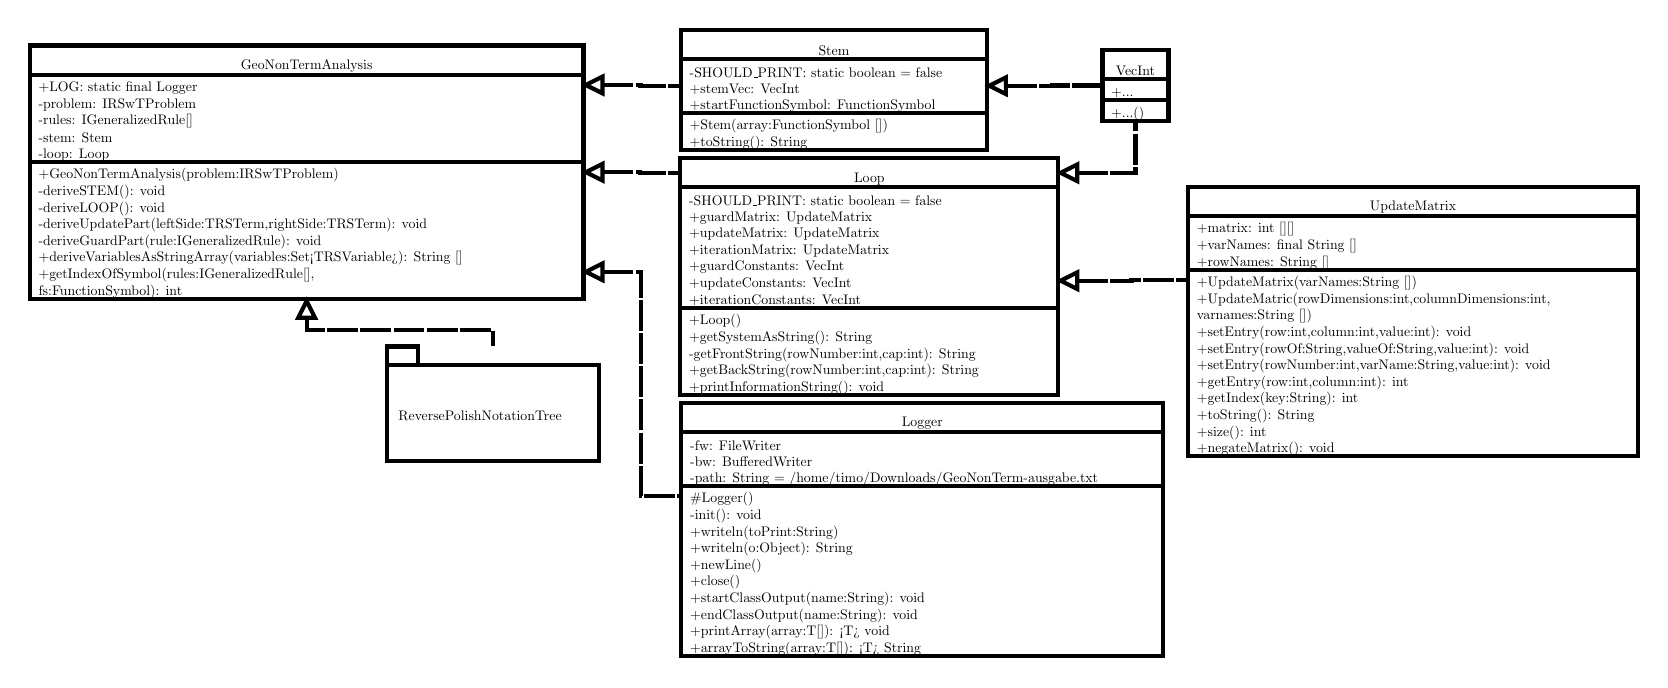
\begin{tikzpicture}[scale=0.5, every node/.style={scale=0.5}]
\pgftransformxscale{1.000000}
\pgftransformyscale{-1.000000}
\definecolor{dialinecolor}{rgb}{0.000000, 0.000000, 0.000000}
\pgfsetstrokecolor{dialinecolor}
\definecolor{dialinecolor}{rgb}{1.000000, 1.000000, 1.000000}
\pgfsetfillcolor{dialinecolor}
\pgfsetlinewidth{0.100000\du}
\pgfsetdash{}{0pt}
\definecolor{dialinecolor}{rgb}{1.000000, 1.000000, 1.000000}
\pgfsetfillcolor{dialinecolor}
\fill (6.851582\du,7.510382\du)--(6.851582\du,8.910382\du)--(33.531582\du,8.910382\du)--(33.531582\du,7.510382\du)--cycle;
\definecolor{dialinecolor}{rgb}{0.000000, 0.000000, 0.000000}
\pgfsetstrokecolor{dialinecolor}
\draw (6.851582\du,7.510382\du)--(6.851582\du,8.910382\du)--(33.531582\du,8.910382\du)--(33.531582\du,7.510382\du)--cycle;
% setfont left to latex
\definecolor{dialinecolor}{rgb}{0.000000, 0.000000, 0.000000}
\pgfsetstrokecolor{dialinecolor}
\node at (20.191582\du,8.510382\du){GeoNonTermAnalysis};
\definecolor{dialinecolor}{rgb}{1.000000, 1.000000, 1.000000}
\pgfsetfillcolor{dialinecolor}
\fill (6.851582\du,8.910382\du)--(6.851582\du,13.110382\du)--(33.531582\du,13.110382\du)--(33.531582\du,8.910382\du)--cycle;
\definecolor{dialinecolor}{rgb}{0.000000, 0.000000, 0.000000}
\pgfsetstrokecolor{dialinecolor}
\draw (6.851582\du,8.910382\du)--(6.851582\du,13.110382\du)--(33.531582\du,13.110382\du)--(33.531582\du,8.910382\du)--cycle;
% setfont left to latex
\definecolor{dialinecolor}{rgb}{0.000000, 0.000000, 0.000000}
\pgfsetstrokecolor{dialinecolor}
\node[anchor=west] at (7.001582\du,9.570382\du){+LOG: static final Logger};
% setfont left to latex
\definecolor{dialinecolor}{rgb}{0.000000, 0.000000, 0.000000}
\pgfsetstrokecolor{dialinecolor}
\node[anchor=west] at (7.001582\du,10.370382\du){-problem: IRSwTProblem};
% setfont left to latex
\definecolor{dialinecolor}{rgb}{0.000000, 0.000000, 0.000000}
\pgfsetstrokecolor{dialinecolor}
\node[anchor=west] at (7.001582\du,11.170382\du){-rules: IGeneralizedRule\ensuremath{[}\ensuremath{]}};
% setfont left to latex
\definecolor{dialinecolor}{rgb}{0.000000, 0.000000, 0.000000}
\pgfsetstrokecolor{dialinecolor}
\node[anchor=west] at (7.001582\du,11.970382\du){-stem: Stem};
% setfont left to latex
\definecolor{dialinecolor}{rgb}{0.000000, 0.000000, 0.000000}
\pgfsetstrokecolor{dialinecolor}
\node[anchor=west] at (7.001582\du,12.770382\du){-loop: Loop};
\definecolor{dialinecolor}{rgb}{1.000000, 1.000000, 1.000000}
\pgfsetfillcolor{dialinecolor}
\fill (6.851582\du,13.110382\du)--(6.851582\du,19.710382\du)--(33.531582\du,19.710382\du)--(33.531582\du,13.110382\du)--cycle;
\definecolor{dialinecolor}{rgb}{0.000000, 0.000000, 0.000000}
\pgfsetstrokecolor{dialinecolor}
\draw (6.851582\du,13.110382\du)--(6.851582\du,19.710382\du)--(33.531582\du,19.710382\du)--(33.531582\du,13.110382\du)--cycle;
% setfont left to latex
\definecolor{dialinecolor}{rgb}{0.000000, 0.000000, 0.000000}
\pgfsetstrokecolor{dialinecolor}
\node[anchor=west] at (7.001582\du,13.770382\du){+GeoNonTermAnalysis(problem:IRSwTProblem)};
% setfont left to latex
\definecolor{dialinecolor}{rgb}{0.000000, 0.000000, 0.000000}
\pgfsetstrokecolor{dialinecolor}
\node[anchor=west] at (7.001582\du,14.570382\du){-deriveSTEM(): void};
% setfont left to latex
\definecolor{dialinecolor}{rgb}{0.000000, 0.000000, 0.000000}
\pgfsetstrokecolor{dialinecolor}
\node[anchor=west] at (7.001582\du,15.370382\du){-deriveLOOP(): void};
% setfont left to latex
\definecolor{dialinecolor}{rgb}{0.000000, 0.000000, 0.000000}
\pgfsetstrokecolor{dialinecolor}
\node[anchor=west] at (7.001582\du,16.170382\du){-deriveUpdatePart(leftSide:TRSTerm,rightSide:TRSTerm): void};
% setfont left to latex
\definecolor{dialinecolor}{rgb}{0.000000, 0.000000, 0.000000}
\pgfsetstrokecolor{dialinecolor}
\node[anchor=west] at (7.001582\du,16.970382\du){-deriveGuardPart(rule:IGeneralizedRule): void};
% setfont left to latex
\definecolor{dialinecolor}{rgb}{0.000000, 0.000000, 0.000000}
\pgfsetstrokecolor{dialinecolor}
\node[anchor=west] at (7.001582\du,17.770382\du){+deriveVariablesAsStringArray(variables:Set<TRSVariable>): String \ensuremath{[}\ensuremath{]}};
% setfont left to latex
\definecolor{dialinecolor}{rgb}{0.000000, 0.000000, 0.000000}
\pgfsetstrokecolor{dialinecolor}
\node[anchor=west] at (7.001582\du,18.570382\du){+getIndexOfSymbol(rules:IGeneralizedRule\ensuremath{[}\ensuremath{]},};
\definecolor{dialinecolor}{rgb}{0.000000, 0.000000, 0.000000}
\pgfsetstrokecolor{dialinecolor}
\node[anchor=west] at (7.001582\du,19.370382\du){                  fs:FunctionSymbol): int};
\pgfsetlinewidth{0.100000\du}
\pgfsetdash{}{0pt}
\definecolor{dialinecolor}{rgb}{1.000000, 1.000000, 1.000000}
\pgfsetfillcolor{dialinecolor}
\fill (38.224621\du,6.749481\du)--(38.224621\du,8.149481\du)--(52.969621\du,8.149481\du)--(52.969621\du,6.749481\du)--cycle;
\definecolor{dialinecolor}{rgb}{0.000000, 0.000000, 0.000000}
\pgfsetstrokecolor{dialinecolor}
\draw (38.224621\du,6.749481\du)--(38.224621\du,8.149481\du)--(52.969621\du,8.149481\du)--(52.969621\du,6.749481\du)--cycle;
% setfont left to latex
\definecolor{dialinecolor}{rgb}{0.000000, 0.000000, 0.000000}
\pgfsetstrokecolor{dialinecolor}
\node at (45.597121\du,7.749481\du){Stem};
\definecolor{dialinecolor}{rgb}{1.000000, 1.000000, 1.000000}
\pgfsetfillcolor{dialinecolor}
\fill (38.224621\du,8.149481\du)--(38.224621\du,10.749481\du)--(52.969621\du,10.749481\du)--(52.969621\du,8.149481\du)--cycle;
\definecolor{dialinecolor}{rgb}{0.000000, 0.000000, 0.000000}
\pgfsetstrokecolor{dialinecolor}
\draw (38.224621\du,8.149481\du)--(38.224621\du,10.749481\du)--(52.969621\du,10.749481\du)--(52.969621\du,8.149481\du)--cycle;
% setfont left to latex
\definecolor{dialinecolor}{rgb}{0.000000, 0.000000, 0.000000}
\pgfsetstrokecolor{dialinecolor}
\node[anchor=west] at (38.374621\du,8.809481\du){-SHOULD\_PRINT: static boolean = false};
% setfont left to latex
\definecolor{dialinecolor}{rgb}{0.000000, 0.000000, 0.000000}
\pgfsetstrokecolor{dialinecolor}
\node[anchor=west] at (38.374621\du,9.609481\du){+stemVec: VecInt};
% setfont left to latex
\definecolor{dialinecolor}{rgb}{0.000000, 0.000000, 0.000000}
\pgfsetstrokecolor{dialinecolor}
\node[anchor=west] at (38.374621\du,10.409481\du){+startFunctionSymbol: FunctionSymbol};
\definecolor{dialinecolor}{rgb}{1.000000, 1.000000, 1.000000}
\pgfsetfillcolor{dialinecolor}
\fill (38.224621\du,10.749481\du)--(38.224621\du,12.549481\du)--(52.969621\du,12.549481\du)--(52.969621\du,10.749481\du)--cycle;
\definecolor{dialinecolor}{rgb}{0.000000, 0.000000, 0.000000}
\pgfsetstrokecolor{dialinecolor}
\draw (38.224621\du,10.749481\du)--(38.224621\du,12.549481\du)--(52.969621\du,12.549481\du)--(52.969621\du,10.749481\du)--cycle;
% setfont left to latex
\definecolor{dialinecolor}{rgb}{0.000000, 0.000000, 0.000000}
\pgfsetstrokecolor{dialinecolor}
\node[anchor=west] at (38.374621\du,11.409481\du){+Stem(array:FunctionSymbol \ensuremath{[}\ensuremath{]})};
% setfont left to latex
\definecolor{dialinecolor}{rgb}{0.000000, 0.000000, 0.000000}
\pgfsetstrokecolor{dialinecolor}
\node[anchor=west] at (38.374621\du,12.209481\du){+toString(): String};
\pgfsetlinewidth{0.100000\du}
\pgfsetdash{}{0pt}
\definecolor{dialinecolor}{rgb}{1.000000, 1.000000, 1.000000}
\pgfsetfillcolor{dialinecolor}
\fill (58.533380\du,7.735360\du)--(58.533380\du,9.135360\du)--(61.715880\du,9.135360\du)--(61.715880\du,7.735360\du)--cycle;
\definecolor{dialinecolor}{rgb}{0.000000, 0.000000, 0.000000}
\pgfsetstrokecolor{dialinecolor}
\draw (58.533380\du,7.735360\du)--(58.533380\du,9.135360\du)--(61.715880\du,9.135360\du)--(61.715880\du,7.735360\du)--cycle;
% setfont left to latex
\definecolor{dialinecolor}{rgb}{0.000000, 0.000000, 0.000000}
\pgfsetstrokecolor{dialinecolor}
\node at (60.124630\du,8.735360\du){VecInt};
\definecolor{dialinecolor}{rgb}{1.000000, 1.000000, 1.000000}
\pgfsetfillcolor{dialinecolor}
\fill (58.533380\du,9.135360\du)--(58.533380\du,10.135360\du)--(61.715880\du,10.135360\du)--(61.715880\du,9.135360\du)--cycle;
\definecolor{dialinecolor}{rgb}{0.000000, 0.000000, 0.000000}
\pgfsetstrokecolor{dialinecolor}
\draw (58.533380\du,9.135360\du)--(58.533380\du,10.135360\du)--(61.715880\du,10.135360\du)--(61.715880\du,9.135360\du)--cycle;
% setfont left to latex
\definecolor{dialinecolor}{rgb}{0.000000, 0.000000, 0.000000}
\pgfsetstrokecolor{dialinecolor}
\node[anchor=west] at (58.683380\du,9.795360\du){+...};
\definecolor{dialinecolor}{rgb}{1.000000, 1.000000, 1.000000}
\pgfsetfillcolor{dialinecolor}
\fill (58.533380\du,10.135360\du)--(58.533380\du,11.135360\du)--(61.715880\du,11.135360\du)--(61.715880\du,10.135360\du)--cycle;
\definecolor{dialinecolor}{rgb}{0.000000, 0.000000, 0.000000}
\pgfsetstrokecolor{dialinecolor}
\draw (58.533380\du,10.135360\du)--(58.533380\du,11.135360\du)--(61.715880\du,11.135360\du)--(61.715880\du,10.135360\du)--cycle;
% setfont left to latex
\definecolor{dialinecolor}{rgb}{0.000000, 0.000000, 0.000000}
\pgfsetstrokecolor{dialinecolor}
\node[anchor=west] at (58.683380\du,10.795360\du){+...()};
\pgfsetlinewidth{0.100000\du}
\pgfsetdash{{1.000000\du}{1.000000\du}}{0\du}
\pgfsetdash{{0.400000\du}{0.400000\du}}{0\du}
\pgfsetmiterjoin
\pgfsetbuttcap
{
\definecolor{dialinecolor}{rgb}{0.000000, 0.000000, 0.000000}
\pgfsetfillcolor{dialinecolor}
% was here!!!
\definecolor{dialinecolor}{rgb}{0.000000, 0.000000, 0.000000}
\pgfsetstrokecolor{dialinecolor}
\draw (33.531582\du,9.410382\du)--(36.278102\du,9.410382\du)--(36.278102\du,9.449481\du)--(38.224621\du,9.449481\du);
}
\definecolor{dialinecolor}{rgb}{0.000000, 0.000000, 0.000000}
\pgfsetstrokecolor{dialinecolor}
\draw (34.443385\du,9.410382\du)--(36.278102\du,9.410382\du)--(36.278102\du,9.449481\du)--(38.224621\du,9.449481\du);
\pgfsetmiterjoin
\definecolor{dialinecolor}{rgb}{1.000000, 1.000000, 1.000000}
\pgfsetfillcolor{dialinecolor}
\fill (34.443385\du,9.010382\du)--(33.643385\du,9.410382\du)--(34.443385\du,9.810382\du)--cycle;
\pgfsetlinewidth{0.100000\du}
\pgfsetdash{}{0pt}
\pgfsetmiterjoin
\definecolor{dialinecolor}{rgb}{0.000000, 0.000000, 0.000000}
\pgfsetstrokecolor{dialinecolor}
\draw (34.443385\du,9.010382\du)--(33.643385\du,9.410382\du)--(34.443385\du,9.810382\du)--cycle;
% setfont left to latex
\pgfsetlinewidth{0.100000\du}
\pgfsetdash{}{0pt}
\definecolor{dialinecolor}{rgb}{1.000000, 1.000000, 1.000000}
\pgfsetfillcolor{dialinecolor}
\fill (38.248518\du,24.714829\du)--(38.248518\du,26.114829\du)--(61.463518\du,26.114829\du)--(61.463518\du,24.714829\du)--cycle;
\definecolor{dialinecolor}{rgb}{0.000000, 0.000000, 0.000000}
\pgfsetstrokecolor{dialinecolor}
\draw (38.248518\du,24.714829\du)--(38.248518\du,26.114829\du)--(61.463518\du,26.114829\du)--(61.463518\du,24.714829\du)--cycle;
% setfont left to latex
\definecolor{dialinecolor}{rgb}{0.000000, 0.000000, 0.000000}
\pgfsetstrokecolor{dialinecolor}
\node at (49.856018\du,25.714829\du){Logger};
\definecolor{dialinecolor}{rgb}{1.000000, 1.000000, 1.000000}
\pgfsetfillcolor{dialinecolor}
\fill (38.248518\du,26.114829\du)--(38.248518\du,28.714829\du)--(61.463518\du,28.714829\du)--(61.463518\du,26.114829\du)--cycle;
\definecolor{dialinecolor}{rgb}{0.000000, 0.000000, 0.000000}
\pgfsetstrokecolor{dialinecolor}
\draw (38.248518\du,26.114829\du)--(38.248518\du,28.714829\du)--(61.463518\du,28.714829\du)--(61.463518\du,26.114829\du)--cycle;
% setfont left to latex
\definecolor{dialinecolor}{rgb}{0.000000, 0.000000, 0.000000}
\pgfsetstrokecolor{dialinecolor}
\node[anchor=west] at (38.398518\du,26.774829\du){-fw: FileWriter};
% setfont left to latex
\definecolor{dialinecolor}{rgb}{0.000000, 0.000000, 0.000000}
\pgfsetstrokecolor{dialinecolor}
\node[anchor=west] at (38.398518\du,27.574829\du){-bw: BufferedWriter};
% setfont left to latex
\definecolor{dialinecolor}{rgb}{0.000000, 0.000000, 0.000000}
\pgfsetstrokecolor{dialinecolor}
\node[anchor=west] at (38.398518\du,28.374829\du){-path: String = /home/timo/Downloads/GeoNonTerm-ausgabe.txt};
\definecolor{dialinecolor}{rgb}{1.000000, 1.000000, 1.000000}
\pgfsetfillcolor{dialinecolor}
\fill (38.248518\du,28.714829\du)--(38.248518\du,36.914829\du)--(61.463518\du,36.914829\du)--(61.463518\du,28.714829\du)--cycle;
\definecolor{dialinecolor}{rgb}{0.000000, 0.000000, 0.000000}
\pgfsetstrokecolor{dialinecolor}
\draw (38.248518\du,28.714829\du)--(38.248518\du,36.914829\du)--(61.463518\du,36.914829\du)--(61.463518\du,28.714829\du)--cycle;
% setfont left to latex
\definecolor{dialinecolor}{rgb}{0.000000, 0.000000, 0.000000}
\pgfsetstrokecolor{dialinecolor}
\node[anchor=west] at (38.398518\du,29.374829\du){\#Logger()};
% setfont left to latex
\definecolor{dialinecolor}{rgb}{0.000000, 0.000000, 0.000000}
\pgfsetstrokecolor{dialinecolor}
\node[anchor=west] at (38.398518\du,30.174829\du){-init(): void};
% setfont left to latex
\definecolor{dialinecolor}{rgb}{0.000000, 0.000000, 0.000000}
\pgfsetstrokecolor{dialinecolor}
\node[anchor=west] at (38.398518\du,30.974829\du){+writeln(toPrint:String)};
% setfont left to latex
\definecolor{dialinecolor}{rgb}{0.000000, 0.000000, 0.000000}
\pgfsetstrokecolor{dialinecolor}
\node[anchor=west] at (38.398518\du,31.774829\du){+writeln(o:Object): String};
% setfont left to latex
\definecolor{dialinecolor}{rgb}{0.000000, 0.000000, 0.000000}
\pgfsetstrokecolor{dialinecolor}
\node[anchor=west] at (38.398518\du,32.574829\du){+newLine()};
% setfont left to latex
\definecolor{dialinecolor}{rgb}{0.000000, 0.000000, 0.000000}
\pgfsetstrokecolor{dialinecolor}
\node[anchor=west] at (38.398518\du,33.374829\du){+close()};
% setfont left to latex
\definecolor{dialinecolor}{rgb}{0.000000, 0.000000, 0.000000}
\pgfsetstrokecolor{dialinecolor}
\node[anchor=west] at (38.398518\du,34.174829\du){+startClassOutput(name:String): void};
% setfont left to latex
\definecolor{dialinecolor}{rgb}{0.000000, 0.000000, 0.000000}
\pgfsetstrokecolor{dialinecolor}
\node[anchor=west] at (38.398518\du,34.974829\du){+endClassOutput(name:String): void};
% setfont left to latex
\definecolor{dialinecolor}{rgb}{0.000000, 0.000000, 0.000000}
\pgfsetstrokecolor{dialinecolor}
\node[anchor=west] at (38.398518\du,35.774829\du){+printArray(array:T\ensuremath{[}\ensuremath{]}): <T> void};
% setfont left to latex
\definecolor{dialinecolor}{rgb}{0.000000, 0.000000, 0.000000}
\pgfsetstrokecolor{dialinecolor}
\node[anchor=west] at (38.398518\du,36.574829\du){+arrayToString(array:T\ensuremath{[}\ensuremath{]}): <T> String};
\pgfsetlinewidth{0.100000\du}
\pgfsetdash{{0.400000\du}{0.400000\du}}{0\du}
\pgfsetdash{{0.400000\du}{0.400000\du}}{0\du}
\pgfsetmiterjoin
\pgfsetbuttcap
{
\definecolor{dialinecolor}{rgb}{0.000000, 0.000000, 0.000000}
\pgfsetfillcolor{dialinecolor}
% was here!!!
\definecolor{dialinecolor}{rgb}{0.000000, 0.000000, 0.000000}
\pgfsetstrokecolor{dialinecolor}
\draw (33.531582\du,18.410382\du)--(36.290050\du,18.410382\du)--(36.290050\du,29.214829\du)--(38.248518\du,29.214829\du);
}
\definecolor{dialinecolor}{rgb}{0.000000, 0.000000, 0.000000}
\pgfsetstrokecolor{dialinecolor}
\draw (34.443385\du,18.410382\du)--(36.290050\du,18.410382\du)--(36.290050\du,29.214829\du)--(38.248518\du,29.214829\du);
\pgfsetmiterjoin
\definecolor{dialinecolor}{rgb}{1.000000, 1.000000, 1.000000}
\pgfsetfillcolor{dialinecolor}
\fill (34.443385\du,18.010382\du)--(33.643385\du,18.410382\du)--(34.443385\du,18.810382\du)--cycle;
\pgfsetlinewidth{0.100000\du}
\pgfsetdash{}{0pt}
\pgfsetmiterjoin
\definecolor{dialinecolor}{rgb}{0.000000, 0.000000, 0.000000}
\pgfsetstrokecolor{dialinecolor}
\draw (34.443385\du,18.010382\du)--(33.643385\du,18.410382\du)--(34.443385\du,18.810382\du)--cycle;
% setfont left to latex
\pgfsetlinewidth{0.100000\du}
\pgfsetdash{{0.400000\du}{0.400000\du}}{0\du}
\pgfsetdash{{0.400000\du}{0.400000\du}}{0\du}
\pgfsetmiterjoin
\pgfsetbuttcap
{
\definecolor{dialinecolor}{rgb}{0.000000, 0.000000, 0.000000}
\pgfsetfillcolor{dialinecolor}
% was here!!!
\definecolor{dialinecolor}{rgb}{0.000000, 0.000000, 0.000000}
\pgfsetstrokecolor{dialinecolor}
\draw (52.969621\du,9.449481\du)--(56.126300\du,9.449481\du)--(56.126300\du,9.435360\du)--(58.482979\du,9.435360\du);
}
\definecolor{dialinecolor}{rgb}{0.000000, 0.000000, 0.000000}
\pgfsetstrokecolor{dialinecolor}
\draw (53.881425\du,9.449481\du)--(56.126300\du,9.449481\du)--(56.126300\du,9.435360\du)--(58.482979\du,9.435360\du);
\pgfsetmiterjoin
\definecolor{dialinecolor}{rgb}{1.000000, 1.000000, 1.000000}
\pgfsetfillcolor{dialinecolor}
\fill (53.881425\du,9.049481\du)--(53.081425\du,9.449481\du)--(53.881425\du,9.849481\du)--cycle;
\pgfsetlinewidth{0.100000\du}
\pgfsetdash{}{0pt}
\pgfsetmiterjoin
\definecolor{dialinecolor}{rgb}{0.000000, 0.000000, 0.000000}
\pgfsetstrokecolor{dialinecolor}
\draw (53.881425\du,9.049481\du)--(53.081425\du,9.449481\du)--(53.881425\du,9.849481\du)--cycle;
% setfont left to latex
\pgfsetlinewidth{0.100000\du}
\pgfsetdash{}{0pt}
\definecolor{dialinecolor}{rgb}{1.000000, 1.000000, 1.000000}
\pgfsetfillcolor{dialinecolor}
\fill (38.197561\du,12.940349\du)--(38.197561\du,14.340349\du)--(56.407561\du,14.340349\du)--(56.407561\du,12.940349\du)--cycle;
\definecolor{dialinecolor}{rgb}{0.000000, 0.000000, 0.000000}
\pgfsetstrokecolor{dialinecolor}
\draw (38.197561\du,12.940349\du)--(38.197561\du,14.340349\du)--(56.407561\du,14.340349\du)--(56.407561\du,12.940349\du)--cycle;
% setfont left to latex
\definecolor{dialinecolor}{rgb}{0.000000, 0.000000, 0.000000}
\pgfsetstrokecolor{dialinecolor}
\node at (47.302561\du,13.940349\du){Loop};
\definecolor{dialinecolor}{rgb}{1.000000, 1.000000, 1.000000}
\pgfsetfillcolor{dialinecolor}
\fill (38.197561\du,14.340349\du)--(38.197561\du,20.140349\du)--(56.407561\du,20.140349\du)--(56.407561\du,14.340349\du)--cycle;
\definecolor{dialinecolor}{rgb}{0.000000, 0.000000, 0.000000}
\pgfsetstrokecolor{dialinecolor}
\draw (38.197561\du,14.340349\du)--(38.197561\du,20.140349\du)--(56.407561\du,20.140349\du)--(56.407561\du,14.340349\du)--cycle;
% setfont left to latex
\definecolor{dialinecolor}{rgb}{0.000000, 0.000000, 0.000000}
\pgfsetstrokecolor{dialinecolor}
\node[anchor=west] at (38.347561\du,15.000349\du){-SHOULD\_PRINT: static boolean = false};
% setfont left to latex
\definecolor{dialinecolor}{rgb}{0.000000, 0.000000, 0.000000}
\pgfsetstrokecolor{dialinecolor}
\node[anchor=west] at (38.347561\du,15.800349\du){+guardMatrix: UpdateMatrix};
% setfont left to latex
\definecolor{dialinecolor}{rgb}{0.000000, 0.000000, 0.000000}
\pgfsetstrokecolor{dialinecolor}
\node[anchor=west] at (38.347561\du,16.600349\du){+updateMatrix: UpdateMatrix};
% setfont left to latex
\definecolor{dialinecolor}{rgb}{0.000000, 0.000000, 0.000000}
\pgfsetstrokecolor{dialinecolor}
\node[anchor=west] at (38.347561\du,17.400349\du){+iterationMatrix: UpdateMatrix};
% setfont left to latex
\definecolor{dialinecolor}{rgb}{0.000000, 0.000000, 0.000000}
\pgfsetstrokecolor{dialinecolor}
\node[anchor=west] at (38.347561\du,18.200349\du){+guardConstants: VecInt};
% setfont left to latex
\definecolor{dialinecolor}{rgb}{0.000000, 0.000000, 0.000000}
\pgfsetstrokecolor{dialinecolor}
\node[anchor=west] at (38.347561\du,19.000349\du){+updateConstants: VecInt};
% setfont left to latex
\definecolor{dialinecolor}{rgb}{0.000000, 0.000000, 0.000000}
\pgfsetstrokecolor{dialinecolor}
\node[anchor=west] at (38.347561\du,19.800349\du){+iterationConstants: VecInt};
\definecolor{dialinecolor}{rgb}{1.000000, 1.000000, 1.000000}
\pgfsetfillcolor{dialinecolor}
\fill (38.197561\du,20.140349\du)--(38.197561\du,24.340349\du)--(56.407561\du,24.340349\du)--(56.407561\du,20.140349\du)--cycle;
\definecolor{dialinecolor}{rgb}{0.000000, 0.000000, 0.000000}
\pgfsetstrokecolor{dialinecolor}
\draw (38.197561\du,20.140349\du)--(38.197561\du,24.340349\du)--(56.407561\du,24.340349\du)--(56.407561\du,20.140349\du)--cycle;
% setfont left to latex
\definecolor{dialinecolor}{rgb}{0.000000, 0.000000, 0.000000}
\pgfsetstrokecolor{dialinecolor}
\node[anchor=west] at (38.347561\du,20.800349\du){+Loop()};
% setfont left to latex
\definecolor{dialinecolor}{rgb}{0.000000, 0.000000, 0.000000}
\pgfsetstrokecolor{dialinecolor}
\node[anchor=west] at (38.347561\du,21.600349\du){+getSystemAsString(): String};
% setfont left to latex
\definecolor{dialinecolor}{rgb}{0.000000, 0.000000, 0.000000}
\pgfsetstrokecolor{dialinecolor}
\node[anchor=west] at (38.347561\du,22.400349\du){-getFrontString(rowNumber:int,cap:int): String};
% setfont left to latex
\definecolor{dialinecolor}{rgb}{0.000000, 0.000000, 0.000000}
\pgfsetstrokecolor{dialinecolor}
\node[anchor=west] at (38.347561\du,23.200349\du){+getBackString(rowNumber:int,cap:int): String};
% setfont left to latex
\definecolor{dialinecolor}{rgb}{0.000000, 0.000000, 0.000000}
\pgfsetstrokecolor{dialinecolor}
\node[anchor=west] at (38.347561\du,24.000349\du){+printInformationString(): void};
\pgfsetlinewidth{0.100000\du}
\pgfsetdash{{0.400000\du}{0.400000\du}}{0\du}
\pgfsetdash{{0.400000\du}{0.400000\du}}{0\du}
\pgfsetmiterjoin
\pgfsetbuttcap
{
\definecolor{dialinecolor}{rgb}{0.000000, 0.000000, 0.000000}
\pgfsetfillcolor{dialinecolor}
% was here!!!
\definecolor{dialinecolor}{rgb}{0.000000, 0.000000, 0.000000}
\pgfsetstrokecolor{dialinecolor}
\draw (33.531582\du,13.610382\du)--(36.264571\du,13.610382\du)--(36.264571\du,13.640349\du)--(38.197561\du,13.640349\du);
}
\definecolor{dialinecolor}{rgb}{0.000000, 0.000000, 0.000000}
\pgfsetstrokecolor{dialinecolor}
\draw (34.443385\du,13.610382\du)--(36.264571\du,13.610382\du)--(36.264571\du,13.640349\du)--(38.197561\du,13.640349\du);
\pgfsetmiterjoin
\definecolor{dialinecolor}{rgb}{1.000000, 1.000000, 1.000000}
\pgfsetfillcolor{dialinecolor}
\fill (34.443385\du,13.210382\du)--(33.643385\du,13.610382\du)--(34.443385\du,14.010382\du)--cycle;
\pgfsetlinewidth{0.100000\du}
\pgfsetdash{}{0pt}
\pgfsetmiterjoin
\definecolor{dialinecolor}{rgb}{0.000000, 0.000000, 0.000000}
\pgfsetstrokecolor{dialinecolor}
\draw (34.443385\du,13.210382\du)--(33.643385\du,13.610382\du)--(34.443385\du,14.010382\du)--cycle;
% setfont left to latex
\pgfsetlinewidth{0.100000\du}
\pgfsetdash{}{0pt}
\definecolor{dialinecolor}{rgb}{1.000000, 1.000000, 1.000000}
\pgfsetfillcolor{dialinecolor}
\fill (62.661558\du,14.305496\du)--(62.661558\du,15.705496\du)--(84.336558\du,15.705496\du)--(84.336558\du,14.305496\du)--cycle;
\definecolor{dialinecolor}{rgb}{0.000000, 0.000000, 0.000000}
\pgfsetstrokecolor{dialinecolor}
\draw (62.661558\du,14.305496\du)--(62.661558\du,15.705496\du)--(84.336558\du,15.705496\du)--(84.336558\du,14.305496\du)--cycle;
% setfont left to latex
\definecolor{dialinecolor}{rgb}{0.000000, 0.000000, 0.000000}
\pgfsetstrokecolor{dialinecolor}
\node at (73.499058\du,15.305496\du){UpdateMatrix};
\definecolor{dialinecolor}{rgb}{1.000000, 1.000000, 1.000000}
\pgfsetfillcolor{dialinecolor}
\fill (62.661558\du,15.705496\du)--(62.661558\du,18.305496\du)--(84.336558\du,18.305496\du)--(84.336558\du,15.705496\du)--cycle;
\definecolor{dialinecolor}{rgb}{0.000000, 0.000000, 0.000000}
\pgfsetstrokecolor{dialinecolor}
\draw (62.661558\du,15.705496\du)--(62.661558\du,18.305496\du)--(84.336558\du,18.305496\du)--(84.336558\du,15.705496\du)--cycle;
% setfont left to latex
\definecolor{dialinecolor}{rgb}{0.000000, 0.000000, 0.000000}
\pgfsetstrokecolor{dialinecolor}
\node[anchor=west] at (62.811558\du,16.365496\du){+matrix: int \ensuremath{[}\ensuremath{]}\ensuremath{[}\ensuremath{]}};
% setfont left to latex
\definecolor{dialinecolor}{rgb}{0.000000, 0.000000, 0.000000}
\pgfsetstrokecolor{dialinecolor}
\node[anchor=west] at (62.811558\du,17.165496\du){+varNames: final String \ensuremath{[}\ensuremath{]}};
% setfont left to latex
\definecolor{dialinecolor}{rgb}{0.000000, 0.000000, 0.000000}
\pgfsetstrokecolor{dialinecolor}
\node[anchor=west] at (62.811558\du,17.965496\du){+rowNames: String \ensuremath{[}\ensuremath{]}};
\definecolor{dialinecolor}{rgb}{1.000000, 1.000000, 1.000000}
\pgfsetfillcolor{dialinecolor}
\fill (62.661558\du,18.305496\du)--(62.661558\du,27.305496\du)--(84.336558\du,27.305496\du)--(84.336558\du,18.305496\du)--cycle;
\definecolor{dialinecolor}{rgb}{0.000000, 0.000000, 0.000000}
\pgfsetstrokecolor{dialinecolor}
\draw (62.661558\du,18.305496\du)--(62.661558\du,27.305496\du)--(84.336558\du,27.305496\du)--(84.336558\du,18.305496\du)--cycle;
% setfont left to latex
\definecolor{dialinecolor}{rgb}{0.000000, 0.000000, 0.000000}
\pgfsetstrokecolor{dialinecolor}
\node[anchor=west] at (62.811558\du,18.965496\du){+UpdateMatrix(varNames:String \ensuremath{[}\ensuremath{]})};
% setfont left to latex
\definecolor{dialinecolor}{rgb}{0.000000, 0.000000, 0.000000}
\pgfsetstrokecolor{dialinecolor}
\node[anchor=west] at (62.811558\du,19.765496\du){+UpdateMatric(rowDimensions:int,columnDimensions:int,};
\definecolor{dialinecolor}{rgb}{0.000000, 0.000000, 0.000000}
\pgfsetstrokecolor{dialinecolor}
\node[anchor=west] at (62.811558\du,20.565496\du){              varnames:String \ensuremath{[}\ensuremath{]})};
% setfont left to latex
\definecolor{dialinecolor}{rgb}{0.000000, 0.000000, 0.000000}
\pgfsetstrokecolor{dialinecolor}
\node[anchor=west] at (62.811558\du,21.365496\du){+setEntry(row:int,column:int,value:int): void};
% setfont left to latex
\definecolor{dialinecolor}{rgb}{0.000000, 0.000000, 0.000000}
\pgfsetstrokecolor{dialinecolor}
\node[anchor=west] at (62.811558\du,22.165496\du){+setEntry(rowOf:String,valueOf:String,value:int): void};
% setfont left to latex
\definecolor{dialinecolor}{rgb}{0.000000, 0.000000, 0.000000}
\pgfsetstrokecolor{dialinecolor}
\node[anchor=west] at (62.811558\du,22.965496\du){+setEntry(rowNumber:int,varName:String,value:int): void};
% setfont left to latex
\definecolor{dialinecolor}{rgb}{0.000000, 0.000000, 0.000000}
\pgfsetstrokecolor{dialinecolor}
\node[anchor=west] at (62.811558\du,23.765496\du){+getEntry(row:int,column:int): int};
% setfont left to latex
\definecolor{dialinecolor}{rgb}{0.000000, 0.000000, 0.000000}
\pgfsetstrokecolor{dialinecolor}
\node[anchor=west] at (62.811558\du,24.565496\du){+getIndex(key:String): int};
% setfont left to latex
\definecolor{dialinecolor}{rgb}{0.000000, 0.000000, 0.000000}
\pgfsetstrokecolor{dialinecolor}
\node[anchor=west] at (62.811558\du,25.365496\du){+toString(): String};
% setfont left to latex
\definecolor{dialinecolor}{rgb}{0.000000, 0.000000, 0.000000}
\pgfsetstrokecolor{dialinecolor}
\node[anchor=west] at (62.811558\du,26.165496\du){+size(): int};
% setfont left to latex
\definecolor{dialinecolor}{rgb}{0.000000, 0.000000, 0.000000}
\pgfsetstrokecolor{dialinecolor}
\node[anchor=west] at (62.811558\du,26.965496\du){+negateMatrix(): void};
\pgfsetlinewidth{0.100000\du}
\pgfsetdash{{0.400000\du}{0.400000\du}}{0\du}
\pgfsetdash{{0.400000\du}{0.400000\du}}{0\du}
\pgfsetmiterjoin
\pgfsetbuttcap
{
\definecolor{dialinecolor}{rgb}{0.000000, 0.000000, 0.000000}
\pgfsetfillcolor{dialinecolor}
% was here!!!
\definecolor{dialinecolor}{rgb}{0.000000, 0.000000, 0.000000}
\pgfsetstrokecolor{dialinecolor}
\draw (56.407561\du,18.840349\du)--(59.934559\du,18.840349\du)--(59.934559\du,18.805496\du)--(62.661558\du,18.805496\du);
}
\definecolor{dialinecolor}{rgb}{0.000000, 0.000000, 0.000000}
\pgfsetstrokecolor{dialinecolor}
\draw (57.319365\du,18.840349\du)--(59.934559\du,18.840349\du)--(59.934559\du,18.805496\du)--(62.661558\du,18.805496\du);
\pgfsetmiterjoin
\definecolor{dialinecolor}{rgb}{1.000000, 1.000000, 1.000000}
\pgfsetfillcolor{dialinecolor}
\fill (57.319365\du,18.440349\du)--(56.519365\du,18.840349\du)--(57.319365\du,19.240349\du)--cycle;
\pgfsetlinewidth{0.100000\du}
\pgfsetdash{}{0pt}
\pgfsetmiterjoin
\definecolor{dialinecolor}{rgb}{0.000000, 0.000000, 0.000000}
\pgfsetstrokecolor{dialinecolor}
\draw (57.319365\du,18.440349\du)--(56.519365\du,18.840349\du)--(57.319365\du,19.240349\du)--cycle;
% setfont left to latex
\pgfsetlinewidth{0.100000\du}
\pgfsetdash{{0.400000\du}{0.400000\du}}{0\du}
\pgfsetdash{{0.400000\du}{0.400000\du}}{0\du}
\pgfsetmiterjoin
\pgfsetbuttcap
{
\definecolor{dialinecolor}{rgb}{0.000000, 0.000000, 0.000000}
\pgfsetfillcolor{dialinecolor}
% was here!!!
\definecolor{dialinecolor}{rgb}{0.000000, 0.000000, 0.000000}
\pgfsetstrokecolor{dialinecolor}
\draw (20.191582\du,19.710382\du)--(20.191582\du,21.234533\du)--(29.156481\du,21.234533\du)--(29.156481\du,21.958684\du);
}
\definecolor{dialinecolor}{rgb}{0.000000, 0.000000, 0.000000}
\pgfsetstrokecolor{dialinecolor}
\draw (20.191582\du,20.622186\du)--(20.191582\du,21.234533\du)--(29.156481\du,21.234533\du)--(29.156481\du,21.958684\du);
\pgfsetmiterjoin
\definecolor{dialinecolor}{rgb}{1.000000, 1.000000, 1.000000}
\pgfsetfillcolor{dialinecolor}
\fill (20.591582\du,20.622186\du)--(20.191582\du,19.822186\du)--(19.791582\du,20.622186\du)--cycle;
\pgfsetlinewidth{0.100000\du}
\pgfsetdash{}{0pt}
\pgfsetmiterjoin
\definecolor{dialinecolor}{rgb}{0.000000, 0.000000, 0.000000}
\pgfsetstrokecolor{dialinecolor}
\draw (20.591582\du,20.622186\du)--(20.191582\du,19.822186\du)--(19.791582\du,20.622186\du)--cycle;
% setfont left to latex
\pgfsetlinewidth{0.100000\du}
\pgfsetdash{}{0pt}
\definecolor{dialinecolor}{rgb}{1.000000, 1.000000, 1.000000}
\pgfsetfillcolor{dialinecolor}
\fill (24.043981\du,22.909081\du)--(24.043981\du,27.509081\du)--(34.268981\du,27.509081\du)--(34.268981\du,22.909081\du)--cycle;
\definecolor{dialinecolor}{rgb}{0.000000, 0.000000, 0.000000}
\pgfsetstrokecolor{dialinecolor}
\draw (24.043981\du,22.909081\du)--(24.043981\du,27.509081\du)--(34.268981\du,27.509081\du)--(34.268981\du,22.909081\du)--cycle;
\definecolor{dialinecolor}{rgb}{1.000000, 1.000000, 1.000000}
\pgfsetfillcolor{dialinecolor}
\fill (24.043981\du,22.009081\du)--(24.043981\du,22.909081\du)--(25.543981\du,22.909081\du)--(25.543981\du,22.009081\du)--cycle;
\definecolor{dialinecolor}{rgb}{0.000000, 0.000000, 0.000000}
\pgfsetstrokecolor{dialinecolor}
\draw (24.043981\du,22.009081\du)--(24.043981\du,22.909081\du)--(25.543981\du,22.909081\du)--(25.543981\du,22.009081\du)--cycle;
% setfont left to latex
\definecolor{dialinecolor}{rgb}{0.000000, 0.000000, 0.000000}
\pgfsetstrokecolor{dialinecolor}
\node[anchor=west] at (24.343981\du,23.741581\du){};
% setfont left to latex
\definecolor{dialinecolor}{rgb}{0.000000, 0.000000, 0.000000}
\pgfsetstrokecolor{dialinecolor}
\node[anchor=west] at (24.343981\du,24.541581\du){};
% setfont left to latex
\definecolor{dialinecolor}{rgb}{0.000000, 0.000000, 0.000000}
\pgfsetstrokecolor{dialinecolor}
\node[anchor=west] at (24.343981\du,25.341581\du){ReversePolishNotationTree};
% setfont left to latex
\definecolor{dialinecolor}{rgb}{0.000000, 0.000000, 0.000000}
\pgfsetstrokecolor{dialinecolor}
\node[anchor=west] at (24.343981\du,26.141581\du){};
% setfont left to latex
\definecolor{dialinecolor}{rgb}{0.000000, 0.000000, 0.000000}
\pgfsetstrokecolor{dialinecolor}
\node[anchor=west] at (24.343981\du,26.941581\du){};
\pgfsetlinewidth{0.100000\du}
\pgfsetdash{{0.400000\du}{0.400000\du}}{0\du}
\pgfsetdash{{0.400000\du}{0.400000\du}}{0\du}
\pgfsetmiterjoin
\pgfsetbuttcap
{
\definecolor{dialinecolor}{rgb}{0.000000, 0.000000, 0.000000}
\pgfsetfillcolor{dialinecolor}
% was here!!!
\definecolor{dialinecolor}{rgb}{0.000000, 0.000000, 0.000000}
\pgfsetstrokecolor{dialinecolor}
\draw (56.407561\du,13.640349\du)--(60.124630\du,13.640349\du)--(60.124630\du,11.135360\du);
}
\definecolor{dialinecolor}{rgb}{0.000000, 0.000000, 0.000000}
\pgfsetstrokecolor{dialinecolor}
\draw (57.319365\du,13.640349\du)--(60.124630\du,13.640349\du)--(60.124630\du,11.135360\du);
\pgfsetmiterjoin
\definecolor{dialinecolor}{rgb}{1.000000, 1.000000, 1.000000}
\pgfsetfillcolor{dialinecolor}
\fill (57.319365\du,13.240349\du)--(56.519365\du,13.640349\du)--(57.319365\du,14.040349\du)--cycle;
\pgfsetlinewidth{0.100000\du}
\pgfsetdash{}{0pt}
\pgfsetmiterjoin
\definecolor{dialinecolor}{rgb}{0.000000, 0.000000, 0.000000}
\pgfsetstrokecolor{dialinecolor}
\draw (57.319365\du,13.240349\du)--(56.519365\du,13.640349\du)--(57.319365\du,14.040349\du)--cycle;
% setfont left to latex
\end{tikzpicture}

			\caption{Das Klassendiagram des Geometrischen Nicht-Terminierungs Ansatz und seinen Komponenten zum besseren Verständnis der notwendigen Programmteile. Stand: 04.07.2017}
			\label{04.07.2017:: GeoNonTerm-classdiagram}
		\end{figure}
\end{itemize}

\myparagraph{Probleme/Offene Fragen}
\begin{enumerate}
	\item brauche ich dann den \emph{STEM} noch?
	\item woher kommt $Y=\begin{pmatrix}
		4 & 3 \\ 0 & 1 
	\end{pmatrix}$?
	\item Muss in der Guard noch alle $>$ zu $<$ umdrehen damit diese einheitlich sind zu der Literatur \answer Gemacht aber ist das richtig?
\end{enumerate}